\documentclass[12pt, a4paper]{article}
\usepackage{color}
\usepackage[margin=1.8cm]{geometry}
\usepackage{graphicx}

\begin{document}
\title{A fine-tuning experiment on beetle dataset}
\author{LE Van Linh}
\date{August 2018}
\maketitle

\begin{abstract}
In this study, we do an experiment of fine-tuning on the beetle dataset: The fine-tuning has been finished on a convolutional neural network (CNN) included three elementary blocks (each elementary block consists of a convolutional layer, a maximum pooling layer, and a dropout layer) followed by two full-connected layers and a dropout layer. The dataset includes the images of five parts of the beetle: left and right mandibles, elytra, head, and thorax. Firstly, the network has been trained with a subset of beetles images (merged from five parts) to obtain the pre-trained model. Secondly, the pre-trained model has been used to fine-tune on the images of each part (of beetle) to obtain the predicted landmarks. The result of this experiment is evaluated by comparing with the last fine-tuning results (ICPRS-18).
\end{abstract}

\section{Method}
This section describes all the component of process.
\subsection{Network}
The network has been used, is the same with the previous studies \cite{}. It includes three elementary blocks followed by two full-connected layers and a dropout layer. In which, each elementary block includes:
\begin{itemize}
	\item A convolutional layer [32, 64, 128]
	\item A maximum pooling layer [$(2 \times 2), (2 \times 2), (2 \times 2)$]
	\item A dropout layer [0.1, 0.2, 0.3]
\end{itemize}
During the training or fine-tuning process, the parameters of the network are set as following:
\begin{itemize}
	\item Optimize method: Nesterov momentum
	\item Learning rate: Adjust from $0.03$ to $0.00001$
	\item Momentum: Adjust from $0.9$ to $0.9999$
	\item Epochs: $10000$
	\item Train split (ratio of validation data): $0.4$ 
	\item Batch size (training and validation): 128
\end{itemize}
\subsection{Dataset}
The dataset includes the images of 5 parts of beetles and $293$ images for each.  To avoid the overfitting during training and fine-tuning, the augmentation methods based on image processing have been applied to each part to increase the number of the images \cite{}.

To have all the predicted landmarks for images, we have applied cross-validation to select the testing data, the remaining images have been used to train and to valid (called fold).
\subsection{Pre-train and fine-tuning model}
The network has been trained with a fold of images which includes the images of 5 parts to provide the pre-trained model. Then, the pre-trained model has been used to fine tune on the images of each part of beetle. Of course, we have also applied cross-validation during the fine-tuning process to obtain the predicted landmarks for all images.

The coordinates of predicted landmarks are evaluated in the same way as the previous studies: Firstly, we compute the distance between the manual coordinates and corresponding predicted coordinates. Then, the average distance on each landmark has been calculated.
\section{Results}
\begin{figure}[h]
	\caption{The distribution of averages distances on each landmark of right mandible}
	\centering
	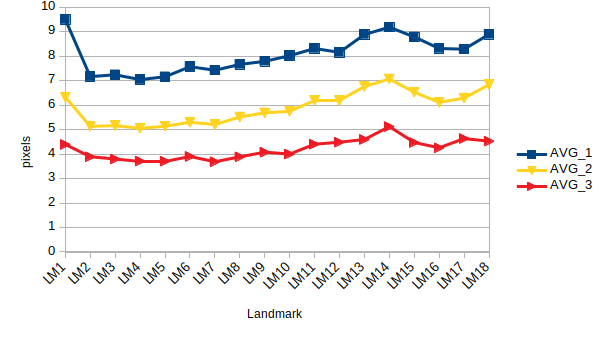
\includegraphics[scale=.71]{images/5parts/md.png}
\end{figure}

\begin{figure}[h]
	\caption{The distribution of averages distances on each landmark of left mandible}
	\centering
	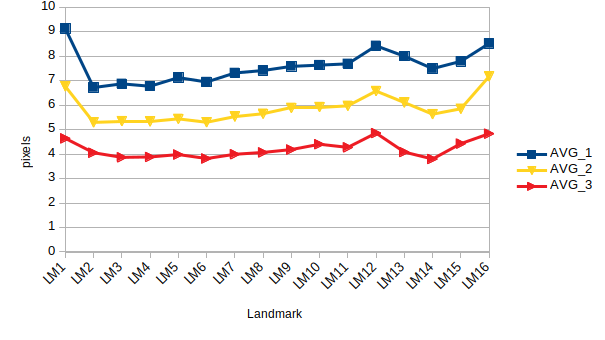
\includegraphics[scale=.71]{images/5parts/mg.png}
\end{figure}

\begin{figure}[!h]
	\caption{The distribution of averages distances on each landmark of head part}
	\centering
	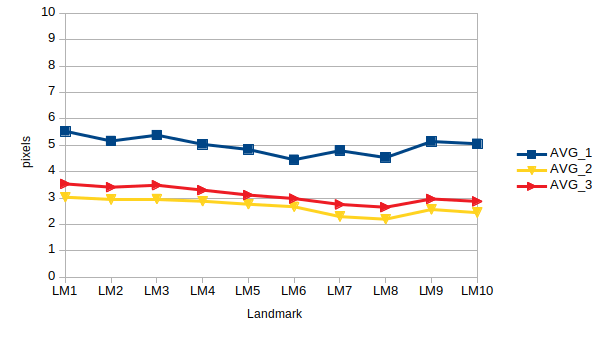
\includegraphics[scale=.8]{images/5parts/tete.png}
\end{figure}

\begin{figure}[!h]
	\caption{The distribution of averages distances on each landmark of thorax part}
	\centering
	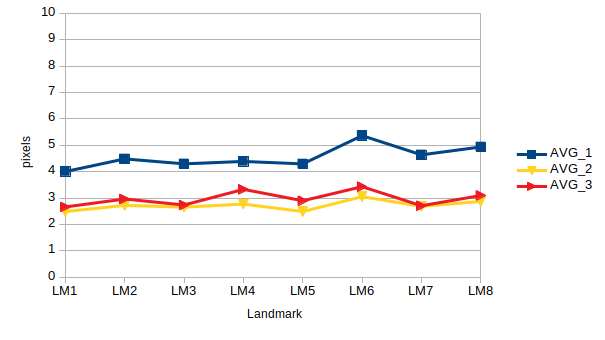
\includegraphics[scale=.8]{images/5parts/pronotum.png}
\end{figure}

\begin{figure}[!h]
	\caption{The distribution of averages distances on each landmark of elytra part}
	\centering
	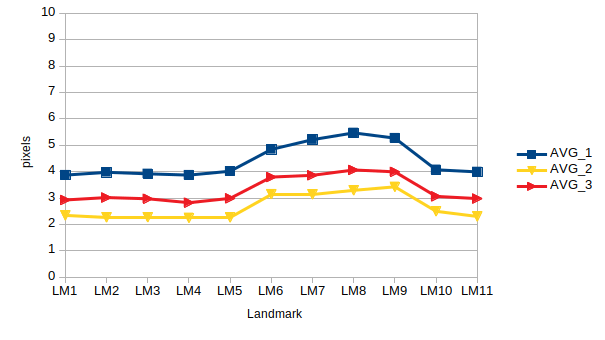
\includegraphics[scale=.8]{images/5parts/elytre.png}
\end{figure}
The figures show the distribution of average distances on each landmark of each part. The blue lines present the average distances per landmark when we train the model from scratch. The yellow lines are the distribution of average distances per landmark when we fine-tune the pre-trained model on each part (the pre-trained model was obtained by training the model on the images of 3 parts: elytra, head, and thorax). The red lines present the average distances per landmarks of this experiment (train model on 5 parts and fine-tune the pre-trained model on each part).

From the figures, we can see that the results of fine-tuning processes have been improved from training from scratch. When we compare the results from the fine-tuning process, we do not see a significant difference between fine-tuning processes on head and thorax part. But the results on the mandible are significantly improved when we train the model with 5 parts and fine-tune on their images. However, the result on the elytra part is in the opposite direction, the distance of this experiment is not as good as the previous one (train with 3 parts and fine-tune on elytra)
\section{Conclusion}
In this study, we have done another experiment of fine-tuning on beetle images. We have trained the model on a subset of images (includes 5 parts), then the pre-trained model has been used to fine-tune on the images of each part to obtain the predicted landmarks. The results show that we do not have a significant difference between fine-tuning processes, i.e. head and thorax but the quality of predicted landmarks on mandibles have been significantly improved.
\end{document}